\documentclass[a4paper, 10pt]{article}
\usepackage[utf8]{inputenc}
\usepackage[spanish]{babel}
\usepackage{hyperref}
\usepackage{tabularx}
\usepackage{inconsolata}
\usepackage{enumitem}
\usepackage{graphicx}

\usepackage{listings}
\usepackage{color}
\usepackage{appendix}
\usepackage{mdframed}
\usepackage{listings}
\usepackage{float}
\usepackage{caption}
\usepackage{subcaption}
\usepackage{subfigure} % subfiguras
\usepackage{anysize} % Soporte para el comando \marginsize

\usepackage{multirow}

\newcommand{\cabeceraSI}[2]{
	\begin{center}
	\begin{tabularx}{\textwidth}{|c c|X|X|X|X}
	\hline
	  \multicolumn{2}{|c|}{\multirow{3}{*}{
\includegraphics[scale=0.10]{../uam.png}}} & \multicolumn{4}{c|}{\bfseries Escuela Politécnica Superior}\\
	  & & \multicolumn{4}{c|}{\bfseries Ingeniería Informática}\\
	  & & \multicolumn{4}{c|}{\bfseries Prácticas de Sistemas Informáticos 2}\\
	\hline
	  \multicolumn{1}{|c|}{\textbf{Grupo}} & 2401 & \multicolumn{1}{|c|}{\textbf{Práctica}} & \multicolumn{1}{>{\centering\arraybackslash}X|}{#1} & \multicolumn{1}{>{\bfseries\centering\arraybackslash}X|}{Fecha} & \multicolumn{1}{c|}{#2}\\
	\hline
	  \multicolumn{2}{|c|}{\textbf{Alumno}} & \multicolumn{4}{l|}{Kasner Tourné, Cristina}\\
	\hline
	  \multicolumn{2}{|c|}{\textbf{Alumno}} & \multicolumn{4}{l|}{Guridi Mateos, Guillermo}\\
	\hline
	\end{tabularx}
	\end{center}
}

\definecolor{mygreen}{rgb}{0,0.6,0}
\definecolor{mygray}{rgb}{0.5,0.5,0.5}
\definecolor{mymauve}{rgb}{0.58,0,0.82}

\makeatletter
\def\@seccntformat#1{%
  \expandafter\ifx\csname c@#1\endcsname\c@section\else
  \csname the#1\endcsname\quad
  \fi}
\makeatother

\newcommand{\tabitem}{\vspace{1mm}~~\llap{\textbullet}~~}

\hypersetup{
    colorlinks=true,
    citecolor=black,
    linkcolor=black,
    urlcolor=blue
}

%% Titulo y autores
\title{Sistemas Informáticos 2\\Práctica 2}
\author{Cristina Kasner Tourné\and Guillermo Guridi Mateos}
\date{\today}

\marginsize{2cm}{2.5cm}{2.5cm}{2.5cm}
%% Documento
\begin{document}

\cabeceraSI{2}{8/04/2015}

\section{Ejercicio 1}
\begin{mdframed} 
Siguiendo todos los pasos anteriores, defina el plan completo de pruebas para realizar las tres 
ejecuciones secuenciales sobre los tres proyectos definidos hasta ahora (P1-base, P1-ws-cli, P1-ejb). 
Adjunte el fichero generado P2.jmx al entregable de la práctica. 
\end{mdframed}
No hemos tenido ningún problema en definir el plan de pruebas tal y como se nos indicaba en el enunciado.

Adjuntamos una imagen con el árbol de resultados.

\begin{figure}[hbtp]
	 	\centering
	 	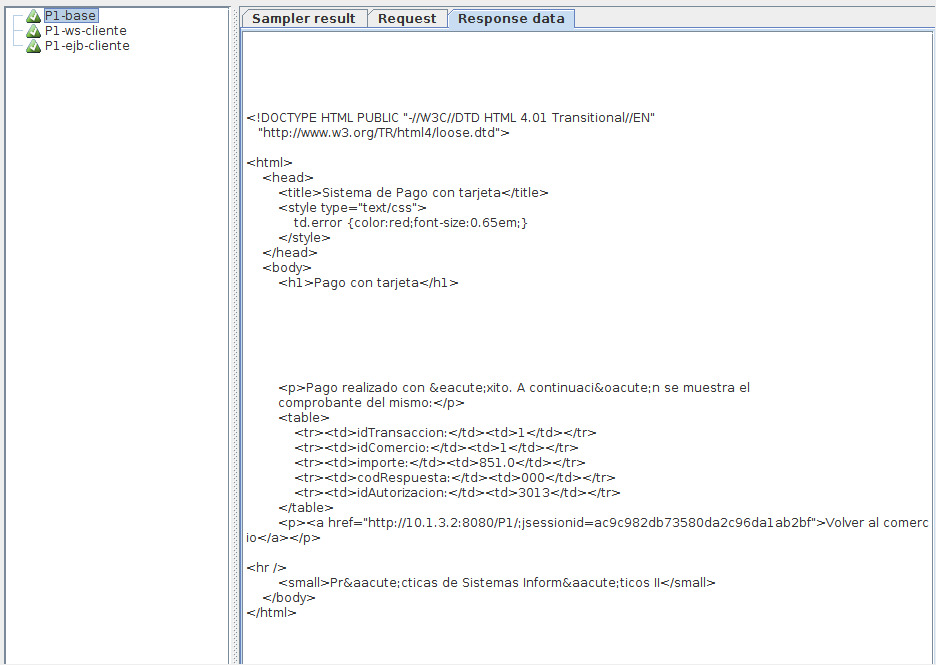
\includegraphics[width=0.8\textwidth]{../../p2/pantallazos/ejemplo_tree_result.png}
	 	\caption {Árbol de resultados}
	 \end{figure}

\pagebreak

\section{Ejercicio 2}
\begin{mdframed} 
Preparar los PCs con el esquema descrito. Para ello:
\begin{itemize}
\item Anote en la memoria de prácticas las direcciones IP asignadas a cada PC. 
\item Detenga el servidor de GlassFish de los PCs físicos 
\item Inicie los servidores GlassFish en las máquinas virtuales 
\item Repliegue todas las aplicaciones o pruebas anteriores (P1-base, P1-ws, etc), para limpiar posibles 
versiones incorrectas. 
\item Revise y modifique si es necesario los ficheros build.properties (propiedad “nombre”) de cada 
versión, de modo que todas las versiones tengan como URL de despliegue las anteriormente 
indicadas (P1-base, P1-ws, P1-ejb). 
\item Despliegue las siguientes prácticas: P1-base, P1-ws, P1-ejb, con el siguiente esquema:
	\begin{itemize}
	\item El destino del despliegue en todos los casos será PC2VM con IP 10.X.Y.2 (as.host o 
as.host.client en P1-ws) 

	\item La base de datos en todos ellos será la de PC1VM con IP 10.X.Y.1 (db.host) 

	\item En el caso particular de P1-ws, el servidor SOAP estará en 10.X.Y.1 (variable 
as.host.server)

	\end{itemize}

\end{itemize}
Tras detener / iniciar todos los elementos indicados, anotar la salida del comando “free” así como un pantallazo del comando “nmon” (pulsaremos la tecla “m” para obtener el estado de la RAM) tanto en las máquinas virtuales como los PCs físicos. Anote sus comentarios en la memoria. 
Pruebe a ejecutar un pago “de calentamiento” por cada uno de los métodos anteriores y verifique que 
funcionan (comprobar resultados en el árbol de resultados). 
\end{mdframed}
 \textbf{Dirección IP asignada al PC 1} : 10.1.3.1 \\
 \textbf{Dirección IP asignada al PC 2} : 10.1.3.2 \\

Tras desplegar y ejecutar free y nmon obtenemos los siguientes resultados:

\begin{figure}[htbp]
\centering
\subfigure[free PC1 antes]{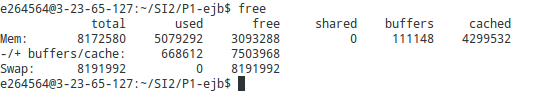
\includegraphics[width=70mm]{../../p2/pantallazos/free_PC_1.png}}
\subfigure[nmon PC1 antes]{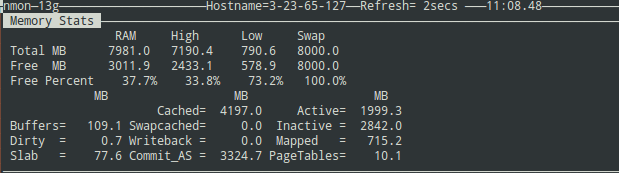
\includegraphics[width=70mm]{../../p2/pantallazos/nmon_pc_1.png}}
\subfigure[free PC1 después]{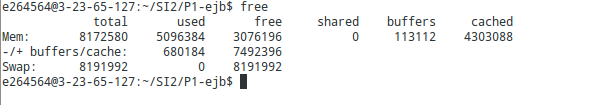
\includegraphics[width=70mm]{../../p2/pantallazos/free_pc1_(glasYpostActiovados).png}}
\subfigure[nmon PC1 después]{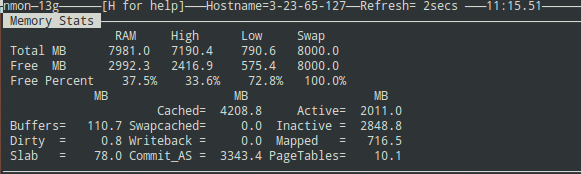
\includegraphics[width=70mm]{../../p2/pantallazos/nmon_pc1_(glasYpostActivados).png}}
\caption{PC 1}
\end{figure}

\begin{figure}[htbp]
\centering
\subfigure[free PC2 antes]{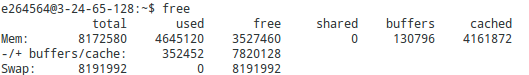
\includegraphics[width=70mm]{../../p2/pantallazos/free_pc_2.png}}
\subfigure[nmon PC2 antes]{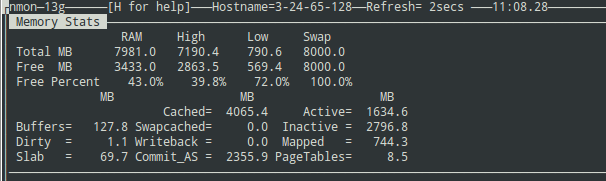
\includegraphics[width=70mm]{../../p2/pantallazos/nmon_pc_2.png}}
\subfigure[free PC2 después]{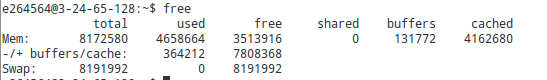
\includegraphics[width=70mm]{../../p2/pantallazos/free_arrancado_PC_2.png}}
\subfigure[nmon PC2 después]{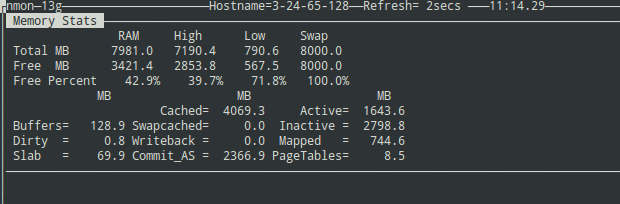
\includegraphics[width=70mm]{../../p2/pantallazos/nmon_arrancado_PC_2.png}}
\caption{PC 2}
\end{figure}

\begin{figure}[htbp]
\centering
\subfigure[free MV1 antes]{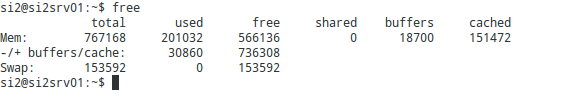
\includegraphics[width=70mm]{../../p2/pantallazos/free_mv_1.png}}
\subfigure[nmon MV1 antes]{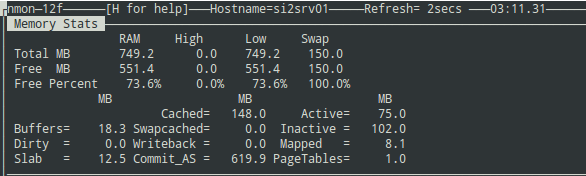
\includegraphics[width=70mm]{../../p2/pantallazos/nmon_mv_1.png}}
\subfigure[free MV1 después]{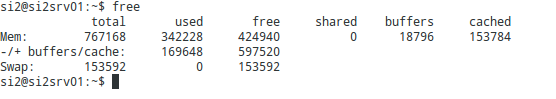
\includegraphics[width=70mm]{../../p2/pantallazos/free_mv1_(freeYpostgresActivados).png}}
\subfigure[nmon MV1 después]{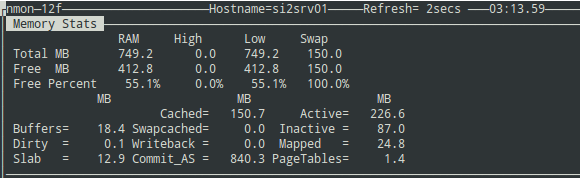
\includegraphics[width=70mm]{../../p2/pantallazos/nmon_mv1_(freeYpostgresActivados).png}}
\caption{máquina virtual 1}
\end{figure}

\begin{figure}[htbp]
\centering
\subfigure[free MV2 antes]{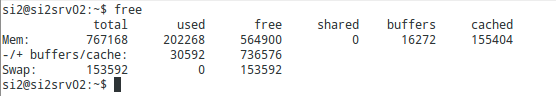
\includegraphics[width=70mm]{../../p2/pantallazos/free_mv_2.png}}
\subfigure[nmon MV2 antes]{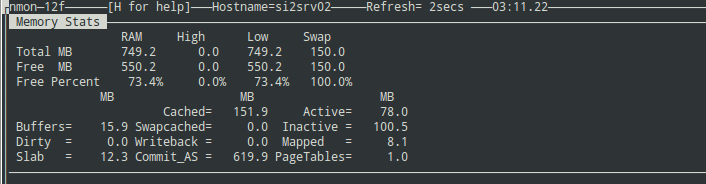
\includegraphics[width=70mm]{../../p2/pantallazos/nmon_mv_2.png}}
\subfigure[free MV2 después]{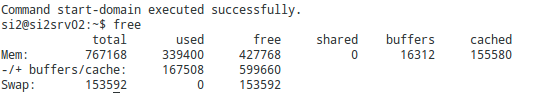
\includegraphics[width=70mm]{../../p2/pantallazos/free_arrancado_mv_2.png}}
\subfigure[nmon MV2 después]{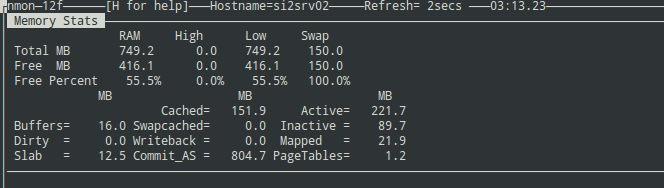
\includegraphics[width=70mm]{../../p2/pantallazos/nmon_arrancado_mv_2.png}}
\caption{máquina virtual 2}
\end{figure}

El comando free nos muestra el uso de memoria actual en el sistema operativo en el que se ejecute. Para este ejercicio nos hemos fijado sobre todo en el porcentaje de memoria libre, comparando las máquinas y PCs sin haber desplegado nada (para ver el consumo base de memoria) con los valores obtenidos tras desplegar toda la aplicación. 

Podemos observar que al hacer free en los PCs, no hay mucha diferencia en el uso de la memoria estando el glassfish y el postgres arrancados o no. Probablemente esto se deba a que los arrancamos dentro de la maquina virtual que probablemente ya tenga parte de la memoria del sistema virtualizado reservada. Ésto se confirma al comprobar que dentro de las máquinas virtuales si que podemos observar un aumento significativo de la memoria usada (entorno a los 140MB).

Nmon, al usarlo solo con 'm' para obtener el mismo tipo de estadísticas nos ofrece las mismas conclusiones.

Adicionalmente, como era de esperar, los valores iniciales son parecidos en las máquinas virtuales entre ellas y en los PCs entre ellos.


\section{Ejercicio 3}
\begin{mdframed} 
Ejecute el plan completo de pruebas sobre las 3 versiones de la práctica, empleando el 
esquema de despliegue descrito anteriormente. Realice la prueba tantas veces como necesite para 
eliminar ruido relacionado con procesos periódicos del sistema operativo, lentitud de la red u otros 
elementos. 

\begin{itemize}
\item Compruebe que efectivamente se han realizado todos los pagos. Es decir, la siguiente 
consulta deberá devolver “3000”:
SELECT COUNT(*) FROM PAGO; 
\end{itemize}  
\end{mdframed}

\begin{figure}[hbtp]
	 	\centering
	 	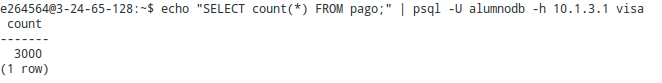
\includegraphics[width=0.8\textwidth]{../../p2/pantallazos/ej3_select_count.png}
	 	\caption{Consulta}
\end{figure}

\begin{mdframed} 
\begin{itemize}
\item Compruebe que ninguna de las peticiones ha producido un error. Para ello revise que la 
columna \,\%Error indique 0\% en todos los casos. 
\end{itemize} 
\end{mdframed}
\begin{figure}[hbtp]
	 	\centering
	 	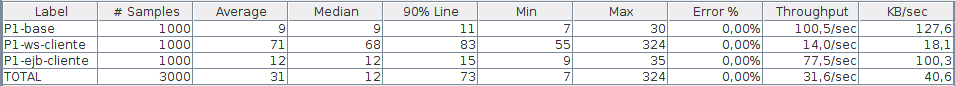
\includegraphics[width=0.8\textwidth]{../../p2/pantallazos/ej3_report.png}
	 	\caption{Comprobación error}
\end{figure}
\begin{mdframed}
\begin{itemize}
Una vez que los resultados han sido satisfactorios: 
\item Anote los resultados del informe agregado en la memoria de la práctica. 
\item Salve el fichero server.log que se encuentra en la ruta glassfish/domains/domain1/logs de 
Glassfish y adjúntelo con la práctica. 
\item Añada a la memoria de prácticas la siguiente información: ¿Cuál de los resultados le parece el 
mejor? ¿Por qué? ¿Qué columna o columnas elegiría para decidir este resultado? 
\end{itemize} 
\end{mdframed} 
El resultado que nos parece mejor es P1-base ya que tiene el mayor Throughput, para eso nos fijamos en la penúltima columna, que es la que nos indica las peticiones completadas por segundo, también sería importante contemplar la columna del percentil 90\% ya que nos garantiza que la mayoría de las peticiones tardarán menos que ese dato. Una vez más gana P1-base, incluso con un poquito más de margen.

Pierde claramente P1-ws, probablemente por las peticiones http extra que tiene que realizar para procesar cada pago.


\section{Ejercicio 4}
\begin{mdframed} 
Adaptar la configuración del servidor de aplicaciones a los valores indicados. Guardar, como 
referencia, la configuración resultante, contenida en el archivo de configuración localizado en la máquina virtual en \$ J2EE\_HOME/domains/domain1/config/domain.xml1. Para obtener la versión correcta de este archivo es necesario detener el servidor de aplicaciones. Incluir este fichero en el entregable de la práctica. Se puede copiar al PC del laboratorio con scp. 
\end{mdframed}

A parte de realizar las modificaciones de configuración creamos un pequeño script (con el comando asadmin) que las modifica por nosotros (excepto las de autodeploy y reload), para poder realizar pruebas en los laboratorios más rapidamente.


\section{Ejercicio 5}
\begin{mdframed} 
Registrar en la hoja de cálculo de resultados los valores de configuración que tienen estos 
parámetros.
\end{mdframed}
\begin{figure}[hbtp]
	 	\centering
	 	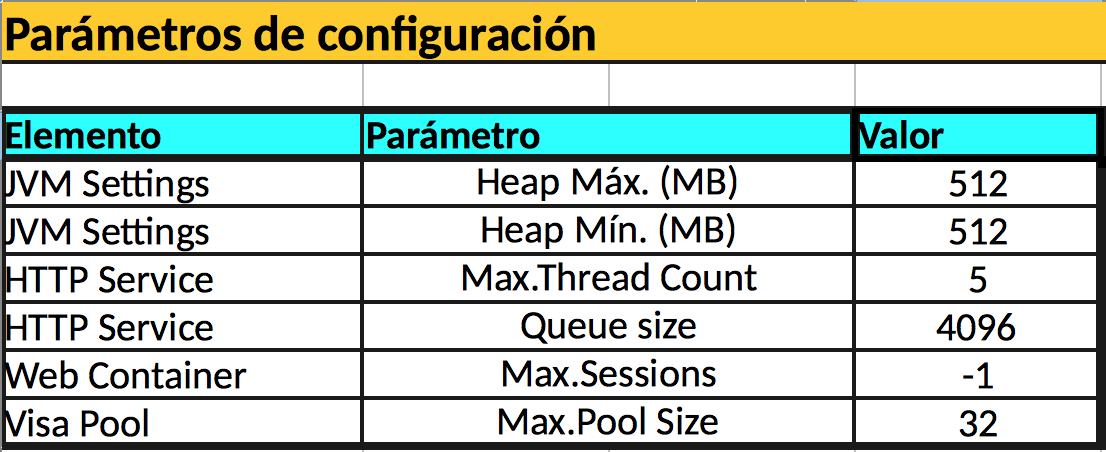
\includegraphics[width=0.8\textwidth]{../../p2/pantallazos/ej5.png}
	 	\caption{}
\end{figure}


\pagebreak
\section{Ejercicio 6}
\begin{mdframed} 
Tras habilitar la monitorización en el servidor, repita la ejecución del plan de pruebas 
anterior. Durante la prueba, vigile cada uno de los elementos de monitorización descritos hasta 
ahora. Responda a las siguientes cuestiones: 
\begin{itemize}
\item A la vista de los resultados, ¿qué elemento de proceso le parece más costosa? ¿Red? ¿CPU? 
¿Acceso a datos? En otras palabras, ¿cuál fue el elemento más utilizado durante la monitorización 
con nmon en un entorno virtual? (CPU, Memoria, disco,…) 
\item ¿Le parece una situación realista la simulada en este ejercicio? ¿Por qué? 
\item Teniendo en cuenta cuál ha sido el elemento más saturado, proponga otro esquema de despliegue 
que resuelva esa situación.
\end{itemize}
\end{mdframed}
Estos fueron los resultados obtenidos:
\begin{figure}[hbtp]
	 	\centering
	 	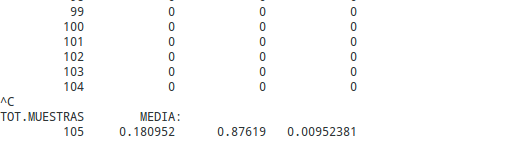
\includegraphics[width=0.8\textwidth]{../../p2/pantallazos/si2_monitor_ej6.png}
	 	\caption{}
\end{figure}
\begin{figure}[hbtp]
	 	\centering
	 	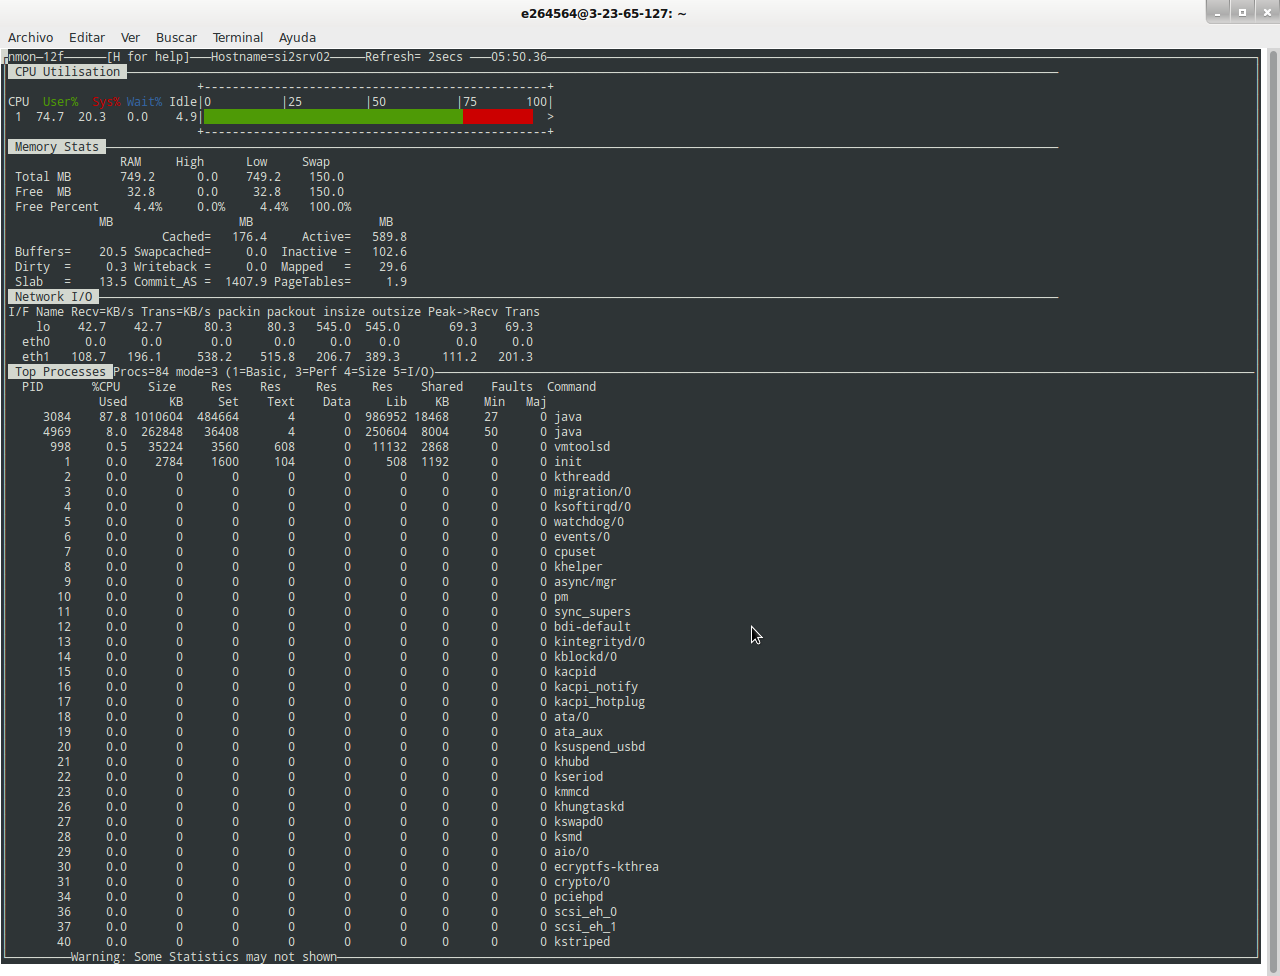
\includegraphics[width=0.8\textwidth]{../../p2/pantallazos/nmon_ej_6_mejor.png}
	 	\caption{nmon durante la prueba de P1-base}
\end{figure}
\begin{figure}[hbtp]
	 	\centering
	 	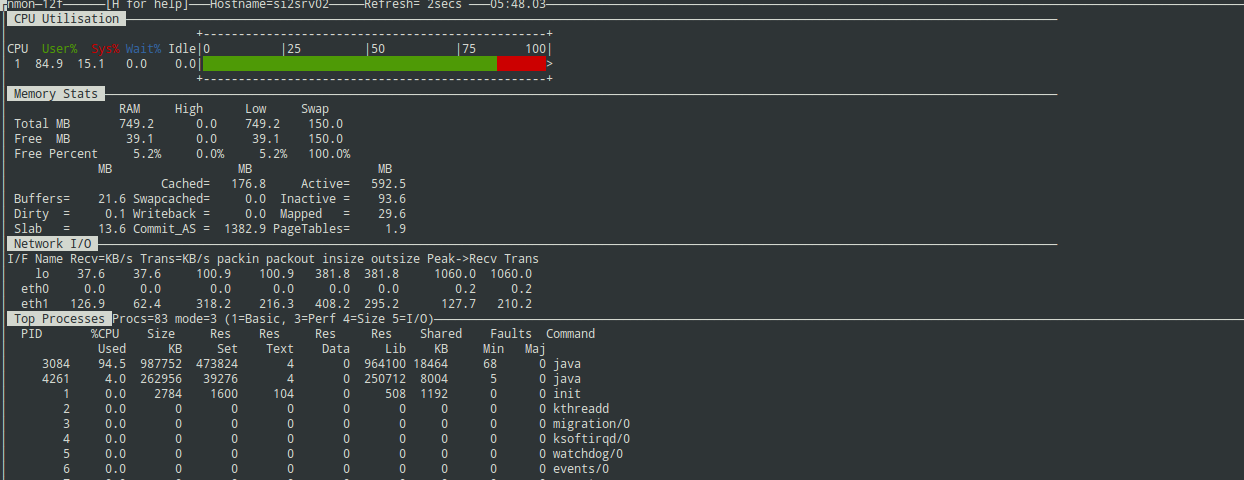
\includegraphics[width=0.8\textwidth]{../../p2/pantallazos/nmon_ej6.png}
	 	\caption{nmon durante la prueba de P1-ws}
\end{figure}

Lo más costoso resulta ser la CPU. Como se puede apreciar en el pantallazo del nmon, java está ocupando el 87\% del procesador y éste ultimo está trabajando en intervalos cercanos al 100\% durante la duración de las pruebas. La memoria se ocupa, pero no parece ser un factor determinante en el rendimiento de este sistema. El uso de red no parece crer ningún cuello de botella ya que los picos máximos de tráfico están en torno a los 100kbps (al exterior y del exterior), lo cual es perfectamente asumible en una red local.

Cabe destacar, como se puede apreciar en el último pantallazo, que durante la prueba de P1-ws se observa un mayor tráfico en la red.

No consideramos esta prueba una situación realista ya que todos los clientes vienen de uno en uno, y son capaces de hacer el pago directamente, en vez de pasar por todo el proceso de la pasarela. Seróia mejor si vinieran concurrentemente y tardaran algo de tiempo en completar los datos del pago, cosa que no se contempla aquí al hacer la petición directamente a procesapago.

Como el elemento más saturado ha sido la CPU, probablemente se debería, o bien, mejorar la cpu de las máquinas de producción, o desplegar varios servidores en paralelo con un load balancer a la entrada. Como la base de datos está en otra máquina no habría ningún problema en duplicar directamente.

\pagebreak
\section{Ejercicio 7}
\begin{mdframed}
Preparar el script de JMeter para su ejecución en el entorno de pruebas. Cambiar la dirección destino del servidor para que acceda al host en el que se encuentra el servidor de aplicaciones. Crear también el directorio datagen en el mismo directorio donde se encuentre el script, y copiar en él el archivo listado.csv, ya que de dicho archivo, al igual que en las prácticas anteriores, se obtienen los datos necesarios para simular el pago.

A continuación, realizar una ejecución del plan de pruebas, con un único usuario, una única ejecución, y un think time bajo (entre 1 y 2 segundos) para verificar que el sistema funciona correctamente. Comprobar, mediante el listener View Results Tree que las peticiones se ejecutan correctamente, no se produce ningún tipo de error y los resultados que se obtienen son los adecuados.
Una vez comprobado que todo el proceso funciona correctamente, desactivar dicho listener del plan de pruebas para que no aumente la carga de proceso de JMeter durante el resto de la prueba.
Este ejercicio no genera información en la memoria de la práctica, realícelo únicamente para garantizar que la siguiente prueba va a funcionar.
\end{mdframed}

Decidimos ejecutar el monitor directamente en la maquina-2 y recoger los resultados de ella cada vez que terminamos una prueba.

\section{Ejercicio 8}
\begin{mdframed}

Obtener la curva de productividad, siguiendo los pasos que se detallan a continuación:
\begin{itemize}
	\item Previamente a la ejecución de la prueba se lanzará una ejecución del script de pruebas (unas 10 ejecuciones de un único usuario) de la que no se tomarán resultados, para iniciar el sistema y preparar medidas consistentes a lo largo de todo al proceso.

	Borrar los resultados de la ejecución anterior. En la barra de acción de JMeter, seleccionar Run $\rightarrow$ Clear All.

	\item Borrar los datos de pagos en la base de datos VISA.
	\item Seleccionar el número de usuarios para la prueba en JMeter (parámetro C de la prueba)
	\item Conmutar en JMeter a la pantalla de presentación de resultados, Aggregate Report.
	\item Ejecutar la prueba. En la barra de accioón de JMeter, seleccionar Run $\rightarrow$ Start.
	\item Ejecutar el programa de monitorización si2-monitor.sh.
	\begin{itemize}
		\item Arrancarlo cuando haya pasado el tiempo definido como rampa de subida de usuarios en JMeter.
		\item Detenerlo cuando esté a punto de terminar la ejecución de la prueba.
		\item Registrar los resultados que proporciona la monitorización en la hoja de cálculo.
	\end{itemize}
	\item Durante el periodo de monitorización anterior, vigilar que los recursos del servidor si2srv02 y del ordenador que se emplea para realizar la prueba no se saturen, mediante inspección del programa de monitorización nmon que se ejecuta en ambas máquinas.
	\item Finalizada la prueba, salvar el resultado de la ejecución del Aggregate Report en un archivo, y registrar en la hoja de cálculo de resultados los valores Average, 90\% line y Throughput para las siguientes peticiones:
	\begin{itemize}
		\item ProcesaPago.
		\item Total.
	\end{itemize}
	Una vez realizadas las iteraciones necesarias para alcanzar la saturación, representar la curva de Throughput versus usuarios.
\end{itemize}

\end{mdframed}

Realizamos las pruebas pedidas empezando en 25 y subiendo de 50 en 50 hasta 775, con la ayuda de un pequeño script para minimizar la influencia del factor humano en los resultados.

\section{Ejercicio 9}
\begin{mdframed} 
Responda a las siguientes cuestiones:
\begin{itemize}
	\item A partir de la curva obtenida, determinar para cuántos usuarios conectados se produce el punto de saturación, cuál es el máximo throughput que se alcanza en el mismo, y el throughput máximo que se obtiene en zona de saturación.
	\item Analizando los valores de monitorización que se han ido obteniendo durante la elaboración de la curva, sugerir el parámetro del servidor de aplicaciones que se cambiaría para obtener el punto de saturación en un número mayor de usuarios.
	\item Realizar el ajuste correspondiente en el servidor de aplicaciones, reiniciarlo y tomar una nueva muestra cercana al punto de saturación. ¿Ha mejorado el rendimiento del sistema? Documente en la memoria de prácticas el cambio realizado y la mejora obtenida.
\end{itemize}
\end{mdframed}

	\begin{figure}[hbtp]
	 	\centering
	 	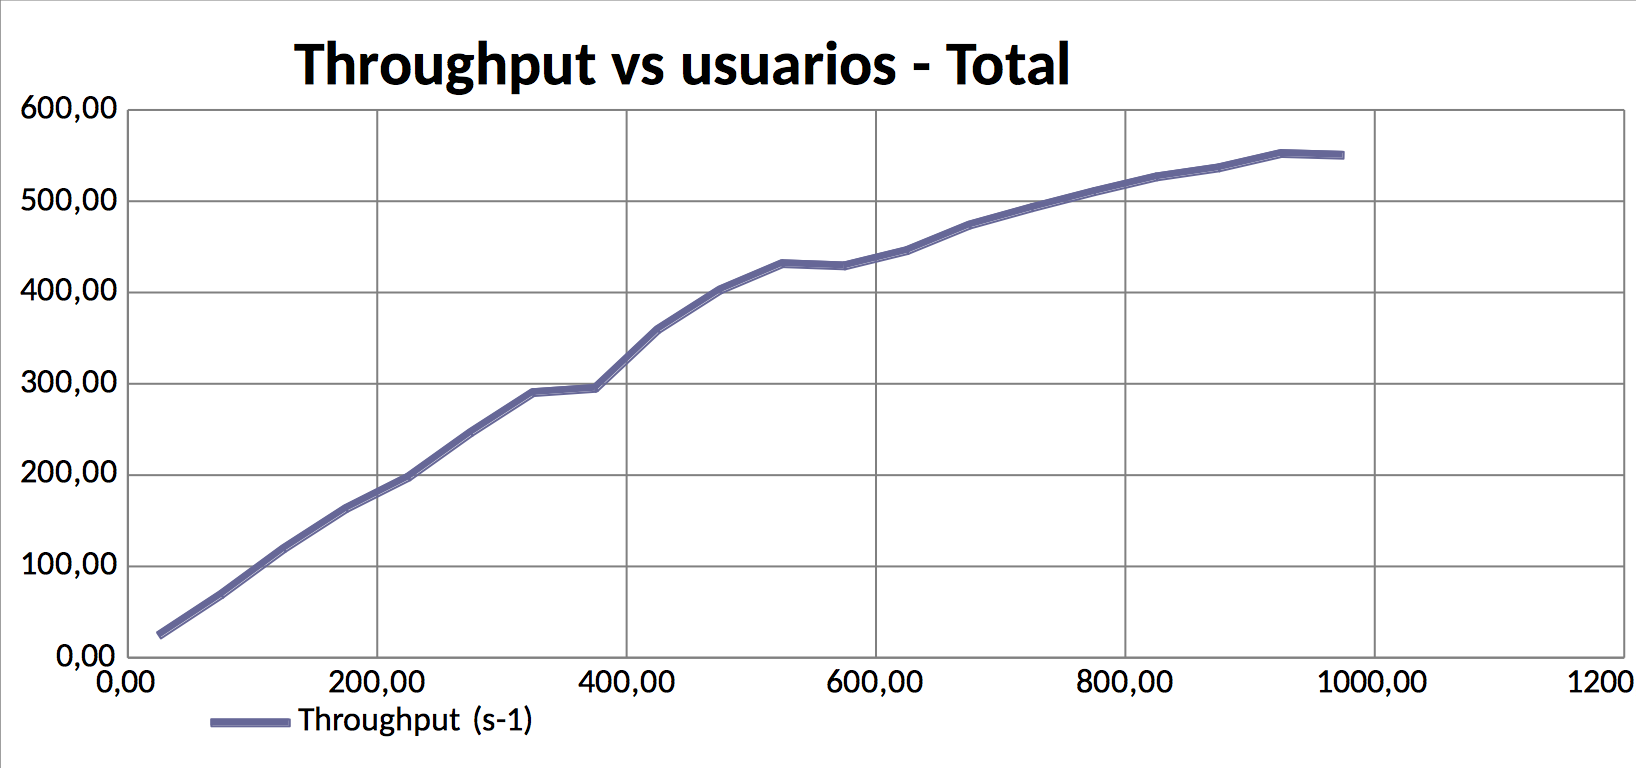
\includegraphics[width=0.8\textwidth]{../../p2/pantallazos/ej9.png}
	\end{figure}

	La curva obtenida es bastante suave, pero estimamos que el punto de saturación se encuentra en torno a los 900 usuarios. A partir de ahí el trhoughput del servidor aumenta bastante más lentamente y hasta decrece un poco.

	El throughput máximo que hemos alcanzado en el punto de saturación está en torno a las 530 peticiones por segundo. En la zona de saturación aumenta hasta las 550 peticiones por segundo.

	Viendo los parámetros del servidor, vemos que la cpu está parada la mayoría del tiempo y que lo que aumenta más rapidamente es el número de peticiones encoladas a la entrada del servidor. Así que decidimos aumentar el número de hilos para recibir las peticiones.

	\pagebreak

	\begin{figure}[hbtp]
	 	\centering
	 	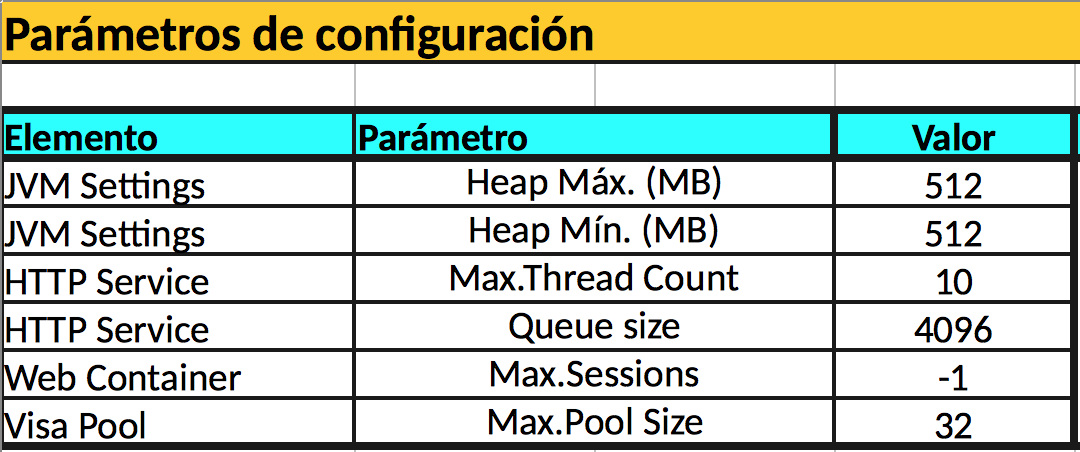
\includegraphics[width=0.8\textwidth]{../../p2/pantallazos/ej9_param.png}
	 	\caption{nuevos parámetros}
	\end{figure}

	Con los nuevos prámetros obtuvimos estos resultados, mucho mejores. Se puede ver como el punto de saturación aumenta más o menos hasta los 1000 usuarios y throughput en saturación hasta 600-610 peticiones por segundo.

	\begin{figure}[hbtp]
	 	\centering
	 	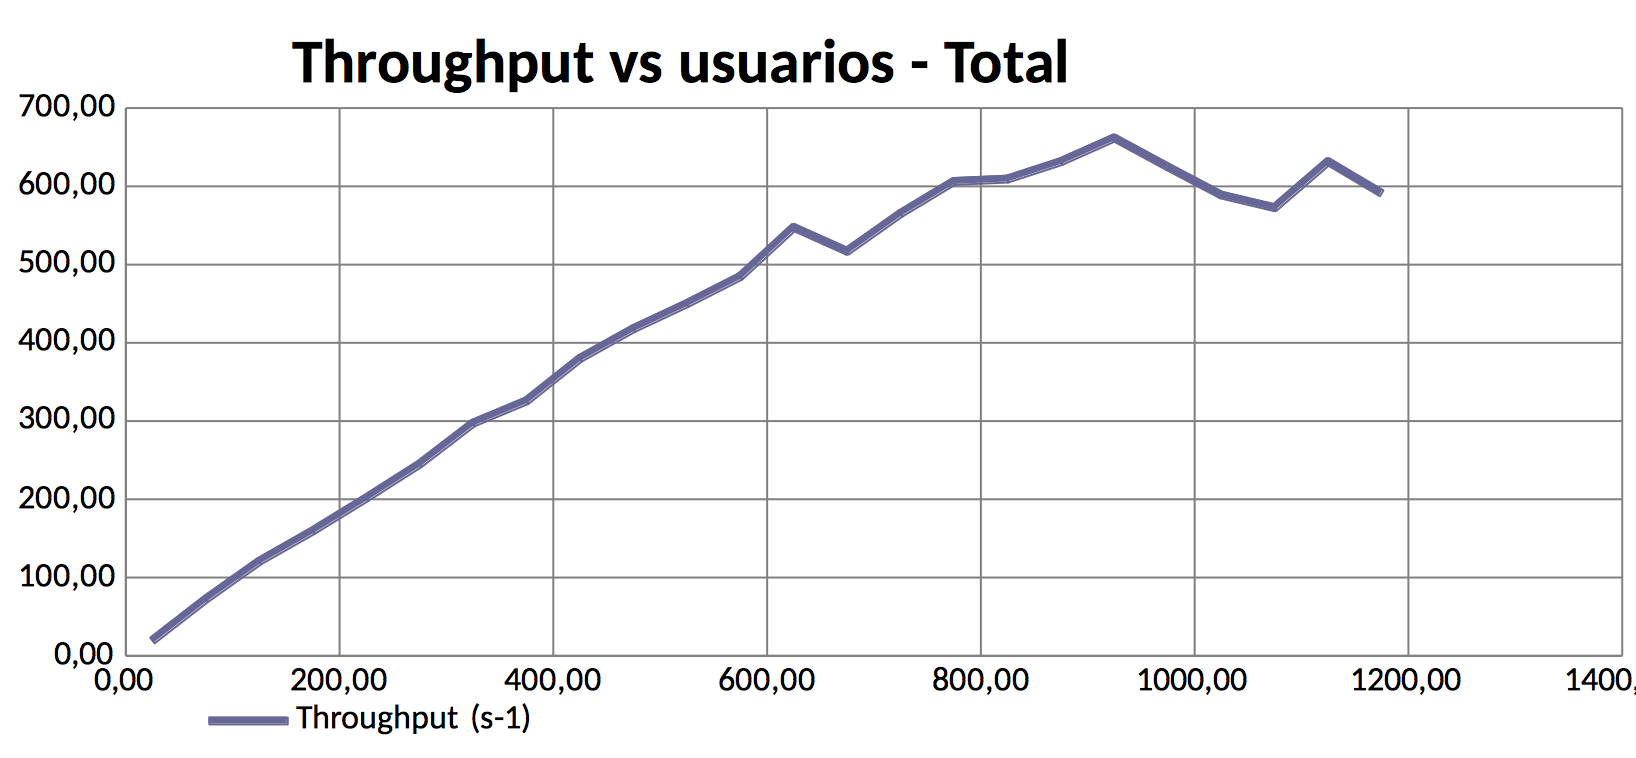
\includegraphics[width=0.8\textwidth]{../../p2/pantallazos/ej9b.png}
	\end{figure}


\end{document}